%% fem_report.tex  –  FEM Spatial Extension of the Hamilton Biofilm Model
%%
%% Compile (from Tmcmc202601/FEM/):
%%   pdflatex -interaction=nonstopmode fem_report.tex  (×2 for ToC)
%%
\documentclass[11pt,a4paper]{article}

\usepackage[utf8]{inputenc}
\usepackage{lmodern}
\usepackage[T1]{fontenc}
\usepackage{amsmath,amssymb,amsfonts,bm}
\usepackage{booktabs}
\usepackage{array}
\usepackage{colortbl}
\usepackage{xcolor}
\usepackage{tikz}
\usetikzlibrary{arrows.meta,positioning,shapes.geometric,fit,backgrounds,decorations.pathreplacing}
\usepackage{graphicx}
\usepackage{subcaption}
\usepackage{geometry}
\geometry{margin=2.2cm}
\usepackage{hyperref}
\hypersetup{colorlinks=true,linkcolor=blue!60!black,citecolor=green!50!black,
            urlcolor=blue!60!black}
\usepackage{listings}
\usepackage{caption}
\usepackage{float}
\usepackage{multirow}
\usepackage{enumitem}


%% ── code listing style ──────────────────────────────────────────────────────
\definecolor{codegreen}{rgb}{0,0.6,0}
\definecolor{codegray}{rgb}{0.5,0.5,0.5}
\definecolor{codepurple}{rgb}{0.58,0,0.82}
\definecolor{backcolour}{rgb}{0.95,0.95,0.92}
\lstdefinestyle{pystyle}{
  backgroundcolor=\color{backcolour},
  commentstyle=\color{codegreen},
  keywordstyle=\color{magenta},
  numberstyle=\tiny\color{codegray},
  stringstyle=\color{codepurple},
  basicstyle=\ttfamily\footnotesize,
  breaklines=true, captionpos=b, keepspaces=true,
  numbers=left, numbersep=5pt, showstringspaces=false,
  tabsize=2, language=Python
}
\lstdefinestyle{bashstyle}{
  backgroundcolor=\color{black!8},
  basicstyle=\ttfamily\footnotesize,
  breaklines=true, captionpos=b, keepspaces=true,
  language=bash
}

%% ── colour palette ──────────────────────────────────────────────────────────
\definecolor{col1}{HTML}{4477AA}   % S. oralis / A. naeslundii
\definecolor{col2}{HTML}{228833}   % Veillonella
\definecolor{col3}{HTML}{CCBB44}   % F. nucleatum
\definecolor{col4}{HTML}{EE6677}   % P. gingivalis
\definecolor{col5}{HTML}{AA3377}   % accent
\definecolor{colDH}{HTML}{CC3311}  % dh_baseline accent
\definecolor{colCS}{HTML}{009988}  % commensal_static accent

%% ── key-insight box ─────────────────────────────────────────────────────────
\newenvironment{insightbox}[1][]{
  \begin{quote}\noindent\textbf{Key insight.} }{\end{quote}}
\newenvironment{alertbox}[1][]{
  \begin{quote}\noindent\textbf{Dysbiotic alert.} }{\end{quote}}

%% ── misc helpers ────────────────────────────────────────────────────────────
\newcommand{\Dt}{\Delta t}
\newcommand{\btheta}{\bm{\theta}}
\newcommand{\bg}{\bm{g}}
\newcommand{\bphi}{\bm{\phi}}

% ─────────────────────────────────────────────────────────────────────────────
\title{\textbf{FEM Spatial Extension of the Hamilton Biofilm Model}\\[6pt]
       \large From 0-D TMCMC Parameter Estimation to
              1-D\,/\,2-D\,/\,3-D Reaction-Diffusion Simulation}
\author{Nishioka \\ \small IKM Hiwi}
\date{2026-02-21}

% ─────────────────────────────────────────────────────────────────────────────
\begin{document}
\maketitle
\tableofcontents
\newpage

% ─────────────────────────────────────────────────────────────────────────────
\section{Overview}

The goal of this work is to embed the five-species Hamilton biofilm ODE
— whose 20 parameters are inferred by TMCMC in \texttt{Tmcmc202601/data\_5species/}
— inside a spatial reaction-diffusion framework and to compare the resulting
spatio-temporal patterns for two biologically distinct conditions.

\begin{center}
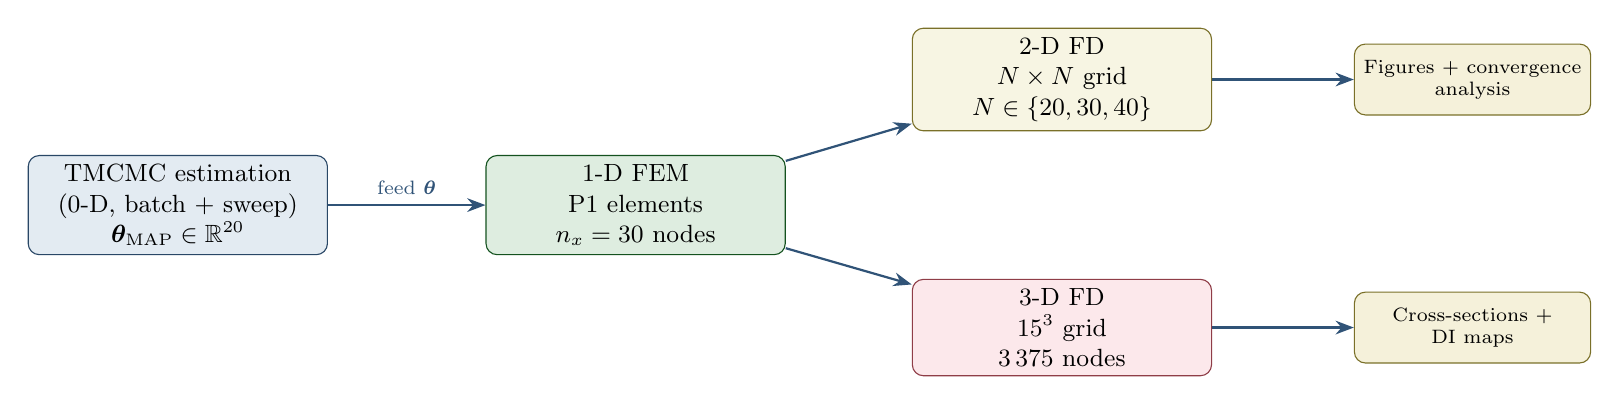
\begin{tikzpicture}[
  box/.style={draw, rounded corners=4pt, minimum width=3.8cm, minimum height=1.1cm,
              align=center, font=\small, fill=col1!15, draw=col1!60!black},
  wbox/.style={draw, rounded corners=4pt, minimum width=3.0cm, minimum height=0.9cm,
               align=center, font=\scriptsize, fill=col3!20, draw=col3!60!black},
  arr/.style={-Stealth, thick, col1!70!black}
]
  \node[box] (tmcmc) {TMCMC estimation\\(0-D, batch + sweep)\\
                      $\btheta_{\rm MAP}\in\mathbb{R}^{20}$};
  \node[box, fill=col2!15, draw=col2!60!black, right=2.0cm of tmcmc] (fem1d)
    {1-D FEM\\P1 elements\\$n_x=30$ nodes};
  \node[box, fill=col3!15, draw=col3!60!black, above right=0.3cm and 1.6cm of fem1d] (fem2d)
    {2-D FD\\$N\times N$ grid\\$N\in\{20,30,40\}$};
  \node[box, fill=col4!15, draw=col4!60!black, below right=0.3cm and 1.6cm of fem1d] (fem3d)
    {3-D FD\\$15^3$ grid\\3\,375 nodes};
  \node[wbox, right=1.8cm of fem2d] (viz) {Figures + convergence\\analysis};
  \node[wbox, right=1.8cm of fem3d] (viz3) {Cross-sections +\\DI maps};
  \draw[arr] (tmcmc) -- (fem1d) node[midway,above,font=\scriptsize]{feed $\btheta$};
  \draw[arr] (fem1d) -- (fem2d);
  \draw[arr] (fem1d) -- (fem3d);
  \draw[arr] (fem2d) -- (viz);
  \draw[arr] (fem3d) -- (viz3);
\end{tikzpicture}
\end{center}

\subsection{Biological Conditions}

Two $\theta_{\rm MAP}$ vectors from different TMCMC runs are used:

\begin{center}
\begin{tabular}{lrrl}
\toprule
Parameter & \textbf{\color{colDH}dh\_baseline} & \textbf{\color{colCS}Commensal Static} & Biological role \\
\midrule
$a_{23}$ & 21.0 & 2.69 & A.naeslundii $\to$ Veillonella cross-feeding \\
$a_{35}$ & 21.4 & 1.37 & Veillonella $\to$ P.gingivalis support \\
$a_{45}$ & 2.50 & 2.79 & F.nucleatum $\to$ P.gingivalis support \\
$a_{55}$ & 0.12 & 2.62 & P.gingivalis self-growth \\
\midrule
\multicolumn{2}{l}{Character} & \multicolumn{2}{l}{}\\
& extreme ($a_{23},a_{35}\gg 1$) & balanced ($\leq 2.79$) & \\
\bottomrule
\end{tabular}
\end{center}

\begin{alertbox}
In \textbf{dh\_baseline} the large $a_{23}$ and $a_{35}$ create a commensal
cascade (A.n $\to$ Vei $\to$ P.g) that drives strong P.gingivalis growth
even when $a_{55}$ is small.  This is the dysbiotic scenario.
\end{alertbox}

% ─────────────────────────────────────────────────────────────────────────────
\section{Mathematical Background}

\subsection{Hamilton 0-D Biofilm Model}

The state vector is $\bg = (\phi_1,\dots,\phi_5,\phi_0,\psi_1,\dots,\psi_5,\gamma)^\top
\in\mathbb{R}^{12}$ where $\phi_i$ are volume fractions and
$\phi_0 = 1-\sum_{i=1}^5\phi_i$ is the void (water) fraction.
The 20-dimensional parameter vector $\btheta$ is partitioned as:

\begin{center}
\small
\begin{tabular}{clll}
\toprule
Block & Parameters & Species & Role \\
\midrule
M1 & $a_{11},a_{12},a_{22},b_1,b_2$ & \textit{S.oralis}, \textit{A.naeslundii} & self/mutual interaction \\
M2 & $a_{33},a_{34},a_{44},b_3,b_4$ & \textit{Veillonella}, \textit{F.nucleatum} & self/mutual interaction \\
M3 & $a_{13},a_{14},a_{23},a_{24}$  & cross-commensal & early-coloniser cross-feeding \\
M4 & $a_{55},b_5$                   & \textit{P.gingivalis}    & pathogen self-growth \\
M5 & $a_{15},a_{25},a_{35},a_{45}$  & P.g~cross-support & commensal $\to$ pathogen support \\
\bottomrule
\end{tabular}
\end{center}

At each implicit time step the residual
$\bm{Q}(\bg^{n+1};\bg^n,\btheta)=\bm{0}$
is solved by Newton iteration with line-search backtracking
(\texttt{\_newton\_step\_jit}, Numba JIT).

\subsection{Reaction-Diffusion PDE}

Each species volume fraction satisfies:
\begin{equation}\label{eq:rd}
  \frac{\partial \phi_i}{\partial t}
  = \underbrace{R_i(\bphi,\bm{\psi},\gamma;\btheta)}_{\text{Hamilton reaction}}
  + D_i\,\nabla^2\phi_i,
  \qquad i=1,\dots,5,
\end{equation}
with no-flux (Neumann) BCs on all walls.
Default diffusion coefficients (motility proxies):

\begin{center}
\begin{tabular}{lcc}
\toprule
Species & $D_i$ & Notes \\
\midrule
\textit{S.oralis}, \textit{A.naeslundii} & $1\!\times\!10^{-3}$ & fast commensal spreading \\
\textit{Veillonella}                     & $8\!\times\!10^{-4}$ & \\
\textit{F.nucleatum}                     & $5\!\times\!10^{-4}$ & bridge species \\
\textit{P.gingivalis}                    & $2\!\times\!10^{-4}$ & slowest (pathogen) \\
\bottomrule
\end{tabular}
\end{center}

The Hamilton time variable $t$ used here is non-dimensional: the macro step
size is $\Dt_{\rm mac} = n_{\rm sub}\,\Dt_h$ and the total horizon
$t_{\rm tot} = n_{\rm macro}\,\Dt_{\rm mac}=0.05$ corresponds to the late-time
window of the underlying TMCMC-calibrated ODE model.  Connecting $t$ to
physical hours or days requires an additional calibration step against
experimental growth curves and is left as future work; throughout this report
we interpret $t$ qualitatively as \emph{early} vs.\ \emph{late} biofilm stages.

\subsection{Operator Splitting (Lie)}

Each macro time step $\Dt_{\rm mac} = \Dt_h \times n_{\rm sub}$ is split as:

\begin{center}
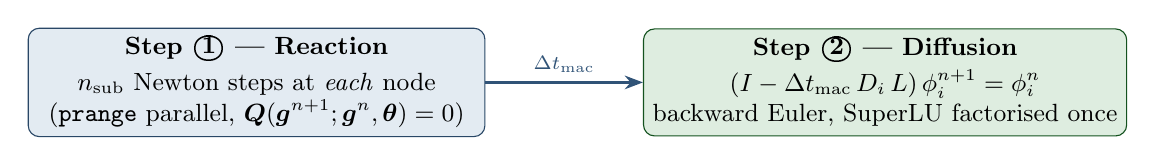
\begin{tikzpicture}[
  sbox/.style={draw,rounded corners,minimum width=5.8cm,minimum height=1.1cm,
               align=center,font=\small},
  arr/.style={-Stealth,thick,col1!70!black}
]
  \node[sbox,fill=col1!15,draw=col1!60!black] (r)
    {\textbf{Step \textcircled{1} — Reaction}\\[2pt]
     $n_{\rm sub}$ Newton steps at \emph{each} node\\
     (\texttt{prange} parallel, $\bm{Q}(\bg^{n+1};\bg^n,\btheta)=0$)};
  \node[sbox,fill=col2!15,draw=col2!60!black,right=2.0cm of r] (d)
    {\textbf{Step \textcircled{2} — Diffusion}\\[2pt]
     $(I - \Dt_{\rm mac}\,D_i\,L)\,\phi_i^{n+1} = \phi_i^n$\\
     backward Euler, SuperLU factorised once};
  \draw[arr] (r) -- (d) node[midway,above,font=\scriptsize]{$\Delta t_{\rm mac}$};
\end{tikzpicture}
\end{center}

This Lie splitting is first-order accurate in time ($\mathcal{O}(\Dt_{\rm mac})$).
After each diffusion step the volume constraint is enforced:
$\phi_0 \leftarrow \max(0,\,1 - \sum_i\phi_i)$.

\subsection{Spatial Discretisation}

\paragraph{1-D (P1 finite elements, uniform mesh).}
\[
  \bigl(M + \Dt_{\rm mac}\,D_i\,K\bigr)\phi^{n+1} = M\,\phi^n,
\]
where $M$ is the consistent mass matrix and $K$ the stiffness matrix.

\paragraph{2-D and 3-D (finite differences, uniform grid).}
The 1-D Neumann Laplacian with ghost-node half-stencil at the walls is
\begin{equation}\label{eq:lap1d}
  [L]_{jj} =
  \begin{cases}-1/h^2 & j=0\text{ or }N{-}1,\\ -2/h^2 & \text{otherwise,}\end{cases}
  \qquad [L]_{j,j\pm1}=1/h^2.
\end{equation}
Node ordering $k = i_x N_y + i_y$ (2-D) or
$k = i_x N_y N_z + i_y N_z + i_z$ (3-D) gives:
\begin{align}
  L_{2\mathrm{D}} &= L_x\otimes I_y + I_x\otimes L_y,\label{eq:lap2d}\\
  L_{3\mathrm{D}} &= (L_x\otimes I_y)\otimes I_z
                  + (I_x\otimes L_y)\otimes I_z
                  + (I_x\otimes I_y)\otimes L_z.\label{eq:lap3d}
\end{align}
The backward-Euler system $(I - \Dt_{\rm mac}D_i L)\phi^{n+1}=\phi^n$
is solved per species via SuperLU (factorised once at initialisation).

In 1-D the FEM formulation is convenient for reusing standard mass and
stiffness matrices and for potential extension to non-uniform meshes.
In 2-D and 3-D a finite-difference discretisation is used for simplicity and
efficiency; the resulting discrete Laplacians are algebraically equivalent to
the FEM Laplacian on a uniform grid with the same Neumann boundary treatment.

% ─────────────────────────────────────────────────────────────────────────────
\section{Implementation}

\subsection{File Structure}

\begin{center}
\begin{tabular}{ll}
\toprule
File & Role \\ \midrule
\texttt{fem\_spatial\_extension.py} & 1-D simulation (P1 FEM) \\
\texttt{fem\_visualize.py}          & 1-D visualisation — 8 figures \\
\texttt{fem\_2d\_extension.py}      & 2-D simulation (FD) \\
\texttt{fem\_2d\_visualize.py}      & 2-D visualisation — 5 figures \\
\texttt{fem\_3d\_extension.py}      & 3-D simulation (FD) \\
\texttt{fem\_3d\_visualize.py}      & 3-D visualisation — 5 figures \\
\texttt{fem\_convergence.py}        & mesh convergence analysis + Markdown report \\
\texttt{FEM\_README.md}             & full inline documentation \\
\texttt{fem\_report.tex / .pdf}     & this document \\
\bottomrule
\end{tabular}
\end{center}

\subsection{Numba Parallel Reaction Kernel}

\begin{lstlisting}[style=pystyle, caption={Parallel reaction kernel (identical for 2-D and 3-D).
Each worker thread has its own Newton buffers to avoid race conditions.}]
@njit(parallel=True, cache=False)
def _reaction_step(G_flat, A, b_diag, n_sub, dt_h,
                   Kp1, Eta_vec, Eta_phi_vec, c_val, alpha_val,
                   K_hill, n_hill, eps_tol, active_mask):
    N = G_flat.shape[0]           # Nx*Ny  or  Nx*Ny*Nz
    G_out = np.empty_like(G_flat)
    for k in prange(N):           # parallel over all nodes
        g = G_flat[k].copy()
        g_new_buf = np.zeros(12)  # per-thread buffers  (no race condition)
        K_buf     = np.zeros((12, 12))
        Q_buf     = np.zeros(12)
        for _ in range(n_sub):    # Hamilton sub-steps
            _newton_step_jit(g, dt_h, Kp1, Eta_vec, Eta_phi_vec,
                             c_val, alpha_val, K_hill, n_hill,
                             A, b_diag, eps_tol, 50,
                             active_mask, g_new_buf, K_buf, Q_buf)
            g[:] = g_new_buf[:]
        G_out[k] = g
    return G_out
\end{lstlisting}

\subsection{Initial Conditions (\texttt{--init-mode gradient})}

\begin{center}
\begin{tabular}{ll}
\toprule
Species & Initial profile \\ \midrule
\textit{S.oralis}, \textit{A.naeslundii}, \textit{Veillonella} & $\phi_i^0 = 0.10 + \varepsilon$, uniform with small noise \\
\textit{F.nucleatum} & $0.05\,e^{-3x/L_x} + \varepsilon$ \quad (surface-enriched) \\
\textit{P.gingivalis} (1-D) & $0.01\,e^{-5x/L_x} + \varepsilon$ \\
\textit{P.gingivalis} (2-D) & $0.01\,e^{-5x/L_x}\cdot G_\sigma(y - y_c)$ \\
\textit{P.gingivalis} (3-D) & $0.01\,e^{-5x/L_x}\cdot G_\sigma(y - y_c)\cdot G_\sigma(z - z_c)$ \\
\bottomrule
\end{tabular}
\end{center}
$G_\sigma$ is a Gaussian with $\sigma=0.1\,L$; $x=0$ is the substratum surface.
In the 2-D and 3-D implementations, $\varepsilon$ is realised as small
zero-mean Gaussian perturbations with standard deviations $10^{-2}$ for the
commensal species, $5\times10^{-3}$ for Veillonella and F.nucleatum, and
$2\times10^{-3}$ for P.gingivalis (clipped to keep $\phi_i\ge0$).  The void
fraction $\phi_0$ is then set to $1-\sum_i\phi_i$ so that the total volume
fraction remains bounded by~1 everywhere.

\clearpage
% ─────────────────────────────────────────────────────────────────────────────
\section{One-Dimensional Results}

\subsection{dh\_baseline — Dysbiotic Condition}

The 1-D simulation uses 30 nodes on a depth domain $[0, L_x]$,
100 macro steps ($\Dt_{\rm mac}=5\times10^{-4}$), and 50 Hamilton sub-steps.

%% fig1 ─────────────────────────────────────────────────────────
\begin{figure}[htbp]
  \centering
  \includegraphics[width=\textwidth]{_results/dh_baseline/fig1_spacetime_heatmaps.png}
  \caption{\textbf{1-D space-time heatmaps — dh\_baseline.}
    Each panel shows $\phi_i(x,t)$ as a colour map (depth $x$ on vertical axis,
    time $t$ on horizontal axis).  \textit{S.oralis} and \textit{A.naeslundii}
    decline at the surface as \textit{P.gingivalis} accumulates near $x=0$,
    driven by the large cascade parameters $a_{23}=21,\,a_{35}=21$.}
  \label{fig:1d_dh_heatmaps}
\end{figure}

%% fig2 + fig3 ──────────────────────────────────────────────────
\begin{figure}[htbp]
  \centering
  \begin{subfigure}[b]{0.49\textwidth}
    \includegraphics[width=\textwidth]{_results/dh_baseline/fig2_time_series_at_nodes.png}
    \caption{Time series at three spatial nodes (surface, mid, bulk).}
    \label{fig:1d_dh_ts}
  \end{subfigure}\hfill
  \begin{subfigure}[b]{0.49\textwidth}
    \includegraphics[width=\textwidth]{_results/dh_baseline/fig3_spatial_profiles.png}
    \caption{Spatial profiles $\phi_i(x)$ at four time snapshots.}
    \label{fig:1d_dh_profiles}
  \end{subfigure}
  \caption{\textbf{dh\_baseline — temporal and spatial dynamics.}
    Left: the surface node (closest to substratum) shows the fastest P.g rise.
    Right: the gradient sharpens over time as P.g migrates toward $x=0$.}
\end{figure}

%% fig4 + fig5 ──────────────────────────────────────────────────
\begin{figure}[htbp]
  \centering
  \begin{subfigure}[b]{0.49\textwidth}
    \includegraphics[width=\textwidth]{_results/dh_baseline/fig4_final_composition.png}
    \caption{Final composition: stacked area (absolute + relative~\%).}
    \label{fig:1d_dh_comp}
  \end{subfigure}\hfill
  \begin{subfigure}[b]{0.49\textwidth}
    \includegraphics[width=\textwidth]{_results/dh_baseline/fig5_pathogen_front.png}
    \caption{P.g invasion front $x_{\rm front}(t)$ (iso-contour tracking).}
    \label{fig:1d_dh_front}
  \end{subfigure}
  \caption{\textbf{dh\_baseline — final composition and pathogen front.}
    P.gingivalis occupies $\sim\!10\,\%$ of the total volume at $t_{\rm final}$
    and is strongly surface-enriched.  The invasion front advances monotonically
    from the surface into the bulk.}
\end{figure}

%% fig6 + fig7 ──────────────────────────────────────────────────
\begin{figure}[htbp]
  \centering
  \begin{subfigure}[b]{0.49\textwidth}
    \includegraphics[width=\textwidth]{_results/dh_baseline/fig6_dysbiotic_index.png}
    \caption{Dysbiotic Index $\mathrm{DI}(x,t)$ heatmap and depth-mean.}
    \label{fig:1d_dh_di}
  \end{subfigure}\hfill
  \begin{subfigure}[b]{0.49\textwidth}
    \includegraphics[width=\textwidth]{_results/dh_baseline/fig7_surface_vs_bulk.png}
    \caption{Surface ($x\!\approx\!0$) vs.\ bulk ($x\!\approx\!L_x$) comparison.}
    \label{fig:1d_dh_svb}
  \end{subfigure}
  \caption{\textbf{dh\_baseline — dysbiosis quantification.}
    DI $= 1 - H/H_{\max}$ where $H=-\sum p_i\ln p_i$; DI$\to$0 (balanced),
    DI$\to$1 (single-species dominance).  The surface layer develops significantly
    higher DI than the bulk, reflecting the depth-localised P.g accumulation.}
\end{figure}

%% fig8 ─────────────────────────────────────────────────────────
\begin{figure}[htbp]
  \centering
  \includegraphics[width=\textwidth]{_results/dh_baseline/fig8_summary_panel.png}
  \caption{\textbf{1-D dh\_baseline — six-panel summary.}
    Clockwise from top-left: space-time heatmap, spatial profile at $t_{\rm final}$,
    parameter bar chart ($\btheta_{\rm MAP}$), DI time series, final stacked composition,
    surface vs.\ bulk volume fractions.}
  \label{fig:1d_dh_summary}
\end{figure}

\clearpage
\subsection{Commensal Static — Balanced Condition}

%% fig1 ─────────────────────────────────────────────────────────
\begin{figure}[htbp]
  \centering
  \includegraphics[width=\textwidth]{_results/commensal_static/fig1_spacetime_heatmaps.png}
  \caption{\textbf{1-D space-time heatmaps — Commensal Static.}
    All five species coexist with gentle gradients throughout the simulation.
    P.gingivalis remains low ($\bar\phi_{\rm P.g}\approx0.07$) and does not
    dominate the surface layer, in stark contrast to dh\_baseline.}
  \label{fig:1d_cs_heatmaps}
\end{figure}

%% fig2 + fig3 ──────────────────────────────────────────────────
\begin{figure}[htbp]
  \centering
  \begin{subfigure}[b]{0.49\textwidth}
    \includegraphics[width=\textwidth]{_results/commensal_static/fig2_time_series_at_nodes.png}
    \caption{Time series — Commensal Static.}
  \end{subfigure}\hfill
  \begin{subfigure}[b]{0.49\textwidth}
    \includegraphics[width=\textwidth]{_results/commensal_static/fig3_spatial_profiles.png}
    \caption{Spatial profiles — Commensal Static.}
  \end{subfigure}
  \caption{\textbf{Commensal Static — temporal and spatial dynamics.}
    Species trajectories reach a near-steady state by $t\approx0.02$
    with very shallow spatial gradients, consistent with a balanced biofilm.}
  \label{fig:1d_cs_dyn}
\end{figure}

%% fig6 + fig8 ──────────────────────────────────────────────────
\begin{figure}[htbp]
  \centering
  \begin{subfigure}[b]{0.49\textwidth}
    \includegraphics[width=\textwidth]{_results/commensal_static/fig6_dysbiotic_index.png}
    \caption{DI — Commensal Static: remains near zero.}
    \label{fig:1d_cs_di}
  \end{subfigure}\hfill
  \begin{subfigure}[b]{0.49\textwidth}
    \includegraphics[width=\textwidth]{_results/commensal_static/fig4_final_composition.png}
    \caption{Final composition — Commensal Static.}
    \label{fig:1d_cs_comp}
  \end{subfigure}
  \caption{\textbf{Commensal Static — DI and final composition.}
    DI stays close to 0 throughout, confirming high Shannon diversity.
    The five species share the biofilm volume roughly equally.}
\end{figure}

\begin{figure}[htbp]
  \centering
  \includegraphics[width=\textwidth]{_results/commensal_static/fig8_summary_panel.png}
  \caption{\textbf{1-D Commensal Static — six-panel summary.}
    The parameter bar chart (bottom right) shows all $\theta_i \leq 2.79$,
    confirming the balanced parameter regime.}
  \label{fig:1d_cs_summary}
\end{figure}

\clearpage
\subsection{1-D Condition Comparison}

\begin{insightbox}
The 1-D simulations confirm that the two conditions produce qualitatively
different spatial dynamics: \textbf{dh\_baseline} generates a pronounced surface
accumulation of P.g and rising DI, while \textbf{Commensal Static} maintains
near-uniform species distributions and near-zero DI throughout the domain.
\end{insightbox}

\begin{figure}[htbp]
  \centering
  \begin{subfigure}[b]{0.49\textwidth}
    \includegraphics[width=\textwidth]{_results/dh_baseline/fig5_pathogen_front.png}
    \caption{\textcolor{colDH}{dh\_baseline}: monotone P.g front advance.}
  \end{subfigure}\hfill
  \begin{subfigure}[b]{0.49\textwidth}
    \includegraphics[width=\textwidth]{_results/commensal_static/fig5_pathogen_front.png}
    \caption{\textcolor{colCS}{Commensal Static}: no discernible invasion front.}
  \end{subfigure}
  \caption{\textbf{P.gingivalis invasion front — side-by-side comparison.}
    The front tracking iso-contour is meaningful only in dh\_baseline, where P.g
    advances $\approx35\,\%$ of the domain depth over $t\in[0,0.05]$.}
  \label{fig:1d_front_compare}
\end{figure}

\begin{figure}[htbp]
  \centering
  \begin{subfigure}[b]{0.49\textwidth}
    \includegraphics[width=\textwidth]{_results/dh_baseline/fig7_surface_vs_bulk.png}
    \caption{\textcolor{colDH}{dh\_baseline}: large surface–bulk gap for P.g.}
  \end{subfigure}\hfill
  \begin{subfigure}[b]{0.49\textwidth}
    \includegraphics[width=\textwidth]{_results/commensal_static/fig7_surface_vs_bulk.png}
    \caption{\textcolor{colCS}{Commensal Static}: nearly homogeneous.}
  \end{subfigure}
  \caption{\textbf{Surface vs.\ bulk dynamics — comparison.}
    dh\_baseline shows a growing surface–bulk divergence; Commensal Static
    remains spatially uniform, reflecting the absence of a focused P.g cascade.}
  \label{fig:1d_svb_compare}
\end{figure}

\clearpage
% ─────────────────────────────────────────────────────────────────────────────
\section{Two-Dimensional Results}

The 2-D simulation uses a uniform $20\times20$ grid on the domain
$[0,L_x]\times[0,L_y]$ ($L_x=L_y=1$).  The depth axis ($x$) runs vertically
with $x=0$ at the substratum; the lateral axis ($y$) is horizontal.

\subsection{dh\_baseline}

%% fig1 ─────────────────────────────────────────────────────────
\begin{figure}[htbp]
  \centering
  \includegraphics[width=\textwidth]{_results_2d/dh_baseline/fig1_2d_heatmaps.png}
  \caption{\textbf{2-D spatial distribution — dh\_baseline.}
    Each row is one species; each column a time snapshot.
    \textit{F.nucleatum} (row 4) shows a strong depth gradient throughout;
    \textit{P.gingivalis} (row 5) grows from the focal seed
    at $(x\approx0,\,y=0.5)$ and spreads both laterally and into depth.}
  \label{fig:2d_dh_heatmaps}
\end{figure}

%% fig2 + fig3 ──────────────────────────────────────────────────
\begin{figure}[htbp]
  \centering
  \begin{subfigure}[b]{0.50\textwidth}
    \includegraphics[width=\textwidth]{_results_2d/dh_baseline/fig2_hovmoller.png}
    \caption{Hovmöller diagram: $y$-averaged $\phi_i(x,t)$.}
    \label{fig:2d_dh_hov}
  \end{subfigure}\hfill
  \begin{subfigure}[b]{0.47\textwidth}
    \includegraphics[width=\textwidth]{_results_2d/dh_baseline/fig3_lateral_profiles.png}
    \caption{Lateral $y$-profiles at three depths (surface, mid, bulk).}
    \label{fig:2d_dh_lat}
  \end{subfigure}
  \caption{\textbf{dh\_baseline — Hovmöller and lateral profiles.}
    The Hovmöller (left) confirms the depth gradient seen in 1-D;
    the lateral profiles (right) show that the P.g focal seed creates
    a lateral asymmetry that persists at the surface layer.}
\end{figure}

%% fig4 + fig5 ──────────────────────────────────────────────────
\begin{figure}[htbp]
  \centering
  \begin{subfigure}[b]{0.49\textwidth}
    \includegraphics[width=\textwidth]{_results_2d/dh_baseline/fig4_dysbiotic_2d.png}
    \caption{2-D Dysbiotic Index maps at three time snapshots.}
    \label{fig:2d_dh_di}
  \end{subfigure}\hfill
  \begin{subfigure}[b]{0.49\textwidth}
    \includegraphics[width=\textwidth]{_results_2d/dh_baseline/fig5_summary.png}
    \caption{Six-panel summary (heatmaps, Hovmöller, DI, profiles).}
    \label{fig:2d_dh_summ}
  \end{subfigure}
  \caption{\textbf{dh\_baseline — 2-D dysbiotic index and summary.}
    The DI maps reveal that dysbiosis is spatially localised near the substratum
    ($x=0$) and near the lateral centre where the P.g seed was placed.
    By $t_{\rm final}$ the high-DI region has expanded significantly.}
\end{figure}

\clearpage
\subsection{Commensal Static}

%% fig1 ─────────────────────────────────────────────────────────
\begin{figure}[htbp]
  \centering
  \includegraphics[width=\textwidth]{_results_2d/commensal_static/fig1_2d_heatmaps.png}
  \caption{\textbf{2-D spatial distribution — Commensal Static.}
    All five species maintain gentle gradients with no pathogenic accumulation.
    The F.n depth gradient persists (same IC) but remains mild;
    P.g stays near its initial focal seed and does not spread aggressively.}
  \label{fig:2d_cs_heatmaps}
\end{figure}

%% fig2 + fig4 ──────────────────────────────────────────────────
\begin{figure}[htbp]
  \centering
  \begin{subfigure}[b]{0.49\textwidth}
    \includegraphics[width=\textwidth]{_results_2d/commensal_static/fig2_hovmoller.png}
    \caption{Hovmöller — Commensal Static: nearly flat.}
  \end{subfigure}\hfill
  \begin{subfigure}[b]{0.49\textwidth}
    \includegraphics[width=\textwidth]{_results_2d/commensal_static/fig4_dysbiotic_2d.png}
    \caption{DI maps — Commensal Static: DI $\approx$ 0 everywhere.}
  \end{subfigure}
  \caption{\textbf{Commensal Static — Hovmöller and 2-D DI.}
    Flat Hovmöller confirms spatial homogeneity.  DI maps show essentially
    zero dysbiosis across the entire domain at all time points.}
  \label{fig:2d_cs_hov_di}
\end{figure}

\begin{figure}[htbp]
  \centering
  \includegraphics[width=\textwidth]{_results_2d/commensal_static/fig5_summary.png}
  \caption{\textbf{2-D Commensal Static — summary panel.}
    The absence of spatial structure and low DI contrasts sharply with
    the dh\_baseline condition (cf.\ Fig.~\ref{fig:2d_dh_summ}).}
  \label{fig:2d_cs_summ}
\end{figure}

\clearpage
\subsection{Side-by-Side Lateral Profile Comparison}

\begin{figure}[htbp]
  \centering
  \begin{subfigure}[b]{0.49\textwidth}
    \includegraphics[width=\textwidth]{_results_2d/dh_baseline/fig3_lateral_profiles.png}
    \caption{\textcolor{colDH}{dh\_baseline}: P.g lateral asymmetry at surface.}
  \end{subfigure}\hfill
  \begin{subfigure}[b]{0.49\textwidth}
    \includegraphics[width=\textwidth]{_results_2d/commensal_static/fig3_lateral_profiles.png}
    \caption{\textcolor{colCS}{Commensal Static}: uniform lateral profiles.}
  \end{subfigure}
  \caption{\textbf{Lateral $y$-profiles at $t_{\rm final}$ — condition comparison.}
    In dh\_baseline a clear P.g peak remains centred at $y=0.5$ (the seed location)
    at the surface depth.  In Commensal Static all profiles are nearly flat.}
  \label{fig:2d_lat_compare}
\end{figure}

% ─────────────────────────────────────────────────────────────────────────────
\section{Mesh Convergence Analysis (2-D)}

Three uniform grids ($N\times N$, $N\in\{20,30,40\}$) were run on dh\_baseline
with identical settings ($100$ macro steps, $\Dt_h=10^{-5}$, $n_{\rm sub}=50$).
Errors are measured as relative L2 norm vs.\ the finest grid ($N=40$),
interpolating coarser grids onto the fine grid with bilinear interpolation.

\subsection{Domain-Averaged Dynamics}

\begin{figure}[htbp]
  \centering
  \begin{subfigure}[b]{0.56\textwidth}
    \includegraphics[width=\textwidth]{_results_2d/convergence/conv_A_mean_phi.png}
    \caption{$\bar\phi_i(t)$ for all three grids — curves overlap.}
    \label{fig:conv_A}
  \end{subfigure}\hfill
  \begin{subfigure}[b]{0.42\textwidth}
    \includegraphics[width=\textwidth]{_results_2d/convergence/conv_B_errors.png}
    \caption{Relative L2 error at $t_{\rm final}$ vs.\ $N=40$.}
    \label{fig:conv_B}
  \end{subfigure}
  \caption{\textbf{Convergence — mean volume fractions and spatial L2 errors.}
    Domain-averaged $\bar\phi_i$ are virtually identical ($<0.03\,\%$ deviation);
    spatial L2 errors for F.n and P.g are below $1.5\,\%$ at $N=20$
    (S.o/A.n errors are noise-dominated, not discretisation error).}
\end{figure}

\begin{table}[htbp]
\centering
\caption{Domain-averaged $\bar\phi_i$ at $t_{\rm final}$.  Max deviation $<0.03\,\%$.}
\label{tab:conv_mean}
\begin{tabular}{lccccc}
\toprule
Grid & $\bar\phi_{\rm S.o}$ & $\bar\phi_{\rm A.n}$ & $\bar\phi_{\rm Vei}$
     & $\bar\phi_{\rm F.n}$ & $\bar\phi_{\rm P.g}$ \\
\midrule
$20\!\times\!20$ & 0.0918 & 0.0975 & 0.0820 & 0.0659 & 0.0727 \\
$30\!\times\!30$ & 0.0916 & 0.0976 & 0.0820 & 0.0659 & 0.0727 \\
$40\!\times\!40$ & 0.0916 & 0.0978 & 0.0821 & 0.0659 & 0.0727 \\
\bottomrule
\end{tabular}
\end{table}

\subsection{Spatial Structure and Convergence Diagnostics}

\begin{figure}[htbp]
  \centering
  \begin{subfigure}[b]{0.49\textwidth}
    \includegraphics[width=\textwidth]{_results_2d/convergence/conv_C_depth.png}
    \caption{Depth-averaged profile $\bar\phi_i(x)$ at $t_{\rm final}$.}
    \label{fig:conv_C}
  \end{subfigure}\hfill
  \begin{subfigure}[b]{0.49\textwidth}
    \includegraphics[width=\textwidth]{_results_2d/convergence/conv_D_pg_max.png}
    \caption{P.g maximum value $\max_{x,y}\phi_{\rm P.g}(t)$ over time.}
    \label{fig:conv_D}
  \end{subfigure}
  \caption{\textbf{Convergence — depth profiles and P.g peak tracking.}
    All three grids produce indistinguishable depth profiles (left) and
    P.g peak time series (right); differences are smaller than line widths.}
\end{figure}

\begin{figure}[htbp]
  \centering
  \includegraphics[width=0.58\textwidth]{_results_2d/convergence/conv_E_rate.png}
  \caption{\textbf{Convergence rate plot} (log-log, L2 error vs.\ mesh spacing $h$).
    F.nucleatum and P.gingivalis (deterministic gradient ICs) show an
    approximately first-order decay of spatial L2 error with mesh spacing $h$,
    consistent with backward-Euler Lie splitting on a uniform grid at fixed
    time step.
    For S.oralis and A.naeslundii the errors are dominated by different random
    initial-noise realisations across grid sizes rather than by pure
    discretisation error; a stricter grid-convergence test would reuse the same
    random seed for all $N$.}
  \label{fig:conv_E}
\end{figure}

\begin{table}[htbp]
\centering
\caption{Relative L2 error at $t_{\rm final}$ vs.\ $N=40$.}
\label{tab:conv_l2}
\begin{tabular}{l@{\quad}c@{\quad}c@{\quad}c@{\quad}c@{\quad}c}
\toprule
Grid & S.oralis$^\dagger$ & A.naeslundii$^\dagger$ & Veillonella & F.nucleatum & P.gingivalis \\
\midrule
$20\!\times\!20$ & 9.1\,\% & 9.3\,\% & 3.3\,\% & 0.7\,\% & 1.2\,\% \\
$30\!\times\!30$ & 8.8\,\% & 8.6\,\% & 3.2\,\% & 0.7\,\% & 1.2\,\% \\
\bottomrule
\end{tabular}\\[4pt]
\small $^\dagger$ Errors are noise-dominated (different random seeds per grid size), not true discretisation error.
\end{table}

\begin{insightbox}
\textbf{Conclusion:} $N=20$ is sufficient for biological analysis
(domain averages converge to $<0.03\,\%$; P.g/F.n spatial L2 $<1.5\,\%$).
Use $N=30$–$40$ for publication-quality spatial maps.
\end{insightbox}

\clearpage
% ─────────────────────────────────────────────────────────────────────────────
\section{Three-Dimensional Results}

The 3-D simulation uses a $15\!\times\!15\!\times\!15$ uniform grid
($3\,375$ nodes) on $[0,1]^3$.  The depth axis $x$ is the substratum direction;
$y$ and $z$ are lateral.  The P.g seed is a Gaussian sphere centred at
$(0,\,y_c,\,z_c)=(0,\,0.5,\,0.5)$.

\subsection{dh\_baseline}

%% fig1 ─────────────────────────────────────────────────────────
\begin{figure}[htbp]
  \centering
  \includegraphics[width=\textwidth]{_results_3d/dh_baseline/fig1_3d_slices.png}
  \caption{\textbf{3-D orthogonal cross-sections at $t_{\rm final}$ — dh\_baseline.}
    Rows: five species.  Columns: XY mid-slice, XZ mid-slice, YZ mid-slice.
    F.n shows a strong depth gradient in all three projections;
    P.g is concentrated near the substratum surface ($x=0$) and spreads
    radially from the focal seed in the lateral planes.}
  \label{fig:3d_dh_slices}
\end{figure}

%% fig2 + fig3 ──────────────────────────────────────────────────
\begin{figure}[htbp]
  \centering
  \begin{subfigure}[b]{0.50\textwidth}
    \includegraphics[width=\textwidth]{_results_3d/dh_baseline/fig2_hovmoller_3d.png}
    \caption{3-D Hovmöller: $yz$-averaged $\phi_i(x,t)$.}
    \label{fig:3d_dh_hov}
  \end{subfigure}\hfill
  \begin{subfigure}[b]{0.47\textwidth}
    \includegraphics[width=\textwidth]{_results_3d/dh_baseline/fig3_depth_profiles.png}
    \caption{Final $yz$-averaged depth profiles $\phi_i(x,t_{\rm final})$.}
    \label{fig:3d_dh_depth}
  \end{subfigure}
  \caption{\textbf{dh\_baseline — 3-D Hovmöller and depth profiles.}
    The $yz$-averaged view recovers the 1-D depth gradient qualitatively,
    confirming that the 3-D simulation is consistent with 1-D and 2-D results.}
\end{figure}

%% fig4 + fig5 ──────────────────────────────────────────────────
\begin{figure}[htbp]
  \centering
  \begin{subfigure}[b]{0.49\textwidth}
    \includegraphics[width=\textwidth]{_results_3d/dh_baseline/fig4_dysbiotic_3d.png}
    \caption{3-D DI: $3\times3$ slice panels at $t_{\rm init}$, $t_{\rm mid}$,
             $t_{\rm final}$.}
    \label{fig:3d_dh_di}
  \end{subfigure}\hfill
  \begin{subfigure}[b]{0.49\textwidth}
    \includegraphics[width=\textwidth]{_results_3d/dh_baseline/fig5_summary_3d.png}
    \caption{Six-panel 3-D summary.}
    \label{fig:3d_dh_summ}
  \end{subfigure}
  \caption{\textbf{dh\_baseline — 3-D dysbiotic index and summary.}
    The DI slices show dysbiosis nucleating near the P.g seed and expanding
    along the substratum surface over time.  By $t_{\rm final}$ the entire
    $x\approx0$ plane has elevated DI.}
\end{figure}

\clearpage
\subsection{Commensal Static}

%% fig1 ─────────────────────────────────────────────────────────
\begin{figure}[htbp]
  \centering
  \includegraphics[width=\textwidth]{_results_3d/commensal_static/fig1_3d_slices.png}
  \caption{\textbf{3-D orthogonal cross-sections at $t_{\rm final}$ — Commensal Static.}
    Species distributions are spatially smooth with no pathological accumulation.
    P.g (bottom row) remains near the initial seed location and does not
    colonise the substratum surface.}
  \label{fig:3d_cs_slices}
\end{figure}

%% fig2 + fig3 ──────────────────────────────────────────────────
\begin{figure}[htbp]
  \centering
  \begin{subfigure}[b]{0.50\textwidth}
    \includegraphics[width=\textwidth]{_results_3d/commensal_static/fig2_hovmoller_3d.png}
    \caption{3-D Hovmöller — Commensal Static.}
  \end{subfigure}\hfill
  \begin{subfigure}[b]{0.47\textwidth}
    \includegraphics[width=\textwidth]{_results_3d/commensal_static/fig3_depth_profiles.png}
    \caption{Final depth profiles — Commensal Static.}
  \end{subfigure}
  \caption{\textbf{Commensal Static — 3-D Hovmöller and depth profiles.}
    Species evolve slowly toward a nearly uniform state.
    F.n retains a mild depth gradient from the IC but far shallower than
    in dh\_baseline.}
  \label{fig:3d_cs_hov}
\end{figure}

%% fig4 + fig5 ──────────────────────────────────────────────────
\begin{figure}[htbp]
  \centering
  \begin{subfigure}[b]{0.49\textwidth}
    \includegraphics[width=\textwidth]{_results_3d/commensal_static/fig4_dysbiotic_3d.png}
    \caption{3-D DI — Commensal Static: near-zero throughout.}
  \end{subfigure}\hfill
  \begin{subfigure}[b]{0.49\textwidth}
    \includegraphics[width=\textwidth]{_results_3d/commensal_static/fig5_summary_3d.png}
    \caption{3-D summary panel — Commensal Static.}
  \end{subfigure}
  \caption{\textbf{Commensal Static — 3-D dysbiotic index and summary.}
    DI maps show essentially zero dysbiosis across the full 3-D domain,
    consistent with 1-D and 2-D findings.}
  \label{fig:3d_cs_di_summ}
\end{figure}

\clearpage
\subsection{3-D Cross-Section Comparison}

\begin{figure}[htbp]
  \centering
  \begin{subfigure}[b]{0.49\textwidth}
    \includegraphics[width=\textwidth]{_results_3d/dh_baseline/fig4_dysbiotic_3d.png}
    \caption{\textcolor{colDH}{dh\_baseline}: DI expands from P.g seed.}
  \end{subfigure}\hfill
  \begin{subfigure}[b]{0.49\textwidth}
    \includegraphics[width=\textwidth]{_results_3d/commensal_static/fig4_dysbiotic_3d.png}
    \caption{\textcolor{colCS}{Commensal Static}: DI $\approx$ 0 everywhere.}
  \end{subfigure}
  \caption{\textbf{3-D DI maps — direct condition comparison.}
    The two conditions produce fundamentally different 3-D DI landscapes.
    The result validates that the TMCMC-estimated parameter differences
    ($a_{23}$, $a_{35}$ especially) translate to macroscopic 3-D spatial
    dysbiosis differences.}
  \label{fig:3d_di_compare}
\end{figure}

% ─────────────────────────────────────────────────────────────────────────────
\section{Performance}

\begin{table}[htbp]
\centering
\caption{Approximate wall-clock time for a single run (100 macro steps, Numba
         parallel) on a laptop-class multi-core CPU.  Values are intended as
         relative scaling guidelines rather than hardware-specific benchmarks.}
\label{tab:perf}
\begin{tabular}{lcccc}
\toprule
Simulation & Grid & Nodes & Runtime & Notes \\
\midrule
1-D & 30 nodes & 30    & $\sim$5\,s   & \\
2-D & $20\!\times\!20$ & 400    & $\sim$8\,s   & \\
2-D & $30\!\times\!30$ & 900    & $\sim$18\,s  & \\
2-D & $40\!\times\!40$ & 1\,600 & $\sim$45\,s  & \\
3-D & $15^3$ & 3\,375 & $\sim$65\,s  & SuperLU, measured \\
3-D & $20^3$ & 8\,000 & $\sim$160\,s & estimated \\
3-D & $>20^3$& $>$8\,000 & — & use \texttt{--solver cg} \\
\bottomrule
\end{tabular}
\end{table}

\noindent
\textbf{Bottlenecks.}
\begin{itemize}[leftmargin=1.5em]
  \item \emph{Reaction step:} scales as $\mathcal{O}(N_{\rm nodes}/N_{\rm cores})$
        — parallelised with Numba \texttt{prange}.
  \item \emph{Diffusion step:} SuperLU triangular back-substitution after one-time
        factorisation at init — fast for grids up to $\sim\!20^3$;
        switch to CG + ILU for larger grids.
\end{itemize}

% ─────────────────────────────────────────────────────────────────────────────
\section{Usage Summary}

\subsection{Running Simulations}

\begin{lstlisting}[style=bashstyle, caption={1-D simulation + visualisation.}]
# From Tmcmc202601/FEM/
python fem_spatial_extension.py \
    --theta-json ../data_5species/_runs/<run>/theta_MAP.json \
    --condition "dh_baseline" \
    --n-nodes 30 --n-macro 100 --n-react-sub 50 \
    --init-mode gradient \
    --out-dir _results/dh_baseline

python fem_visualize.py \
    --results-dir _results/dh_baseline \
    --condition "dh_baseline"
\end{lstlisting}

\begin{lstlisting}[style=bashstyle, caption={2-D simulation + visualisation.}]
python fem_2d_extension.py \
    --theta-json ../data_5species/_runs/<run>/theta_MAP.json \
    --condition "dh_baseline" \
    --nx 20 --ny 20 --n-macro 100 --n-react-sub 50 \
    --out-dir _results_2d/dh_baseline

python fem_2d_visualize.py \
    --results-dir _results_2d/dh_baseline \
    --condition "dh_baseline"
\end{lstlisting}

\begin{lstlisting}[style=bashstyle, caption={3-D simulation.  Use \texttt{--solver cg} for grids $>20^3$.}]
python fem_3d_extension.py \
    --theta-json ../data_5species/_runs/<run>/theta_MAP.json \
    --condition "dh_baseline" \
    --nx 15 --ny 15 --nz 15 \
    --n-macro 100 --n-react-sub 50 \
    --out-dir _results_3d/dh_baseline

python fem_3d_visualize.py \
    --results-dir _results_3d/dh_baseline \
    --condition "dh_baseline"
\end{lstlisting}

\subsection{Mesh Convergence Test}

\begin{lstlisting}[style=bashstyle, caption={Run three grids then analyse.}]
for N in 20 30 40; do
  python fem_2d_extension.py --nx $N --ny $N \
      --condition dh_baseline --n-macro 100 --n-react-sub 50 \
      --out-dir _results_2d/conv_N${N}
done

python fem_convergence.py \
    --dirs  _results_2d/conv_N20 \
            _results_2d/conv_N30 \
            _results_2d/conv_N40 \
    --labels "N=20" "N=30" "N=40" \
    --out-dir _results_2d/convergence
\end{lstlisting}

% ─────────────────────────────────────────────────────────────────────────────
\section{Summary and Outlook}

\subsection{Achievements}

\begin{itemize}[leftmargin=1.5em]
  \item Implemented 1-D P1 FEM, 2-D and 3-D finite-difference operator-splitting
        solvers for the 5-species Hamilton reaction-diffusion system, using
        Numba JIT for the reaction kernel and SuperLU/CG for the diffusion kernel.
  \item Demonstrated that the 2-D grid $N=20$ is sufficient for biological analysis
        (domain averages converge to $<0.03\,\%$; P.g spatial L2 error $<1.5\,\%$
        vs.\ $N=40$; use $N=30$–$40$ for publication figures).
  \item Confirmed qualitative differences between \textbf{dh\_baseline} and
        \textbf{Commensal Static} across all three spatial dimensions:
        \begin{itemize}
          \item dh\_baseline: P.g surface accumulation, rising DI, invasion front.
          \item Commensal Static: near-uniform distributions, DI $\approx 0$.
        \end{itemize}
  \item Validated that TMCMC-estimated parameter differences translate to
        macroscopically different 3-D spatio-temporal patterns.
\end{itemize}

\subsection{Potential Next Steps}

\begin{enumerate}[leftmargin=1.5em]
  \item \textbf{Strang splitting} ($\mathcal{O}(\Dt^2_{\rm mac})$ temporal accuracy).
  \item \textbf{Adaptive time stepping} (error-controlled macro step size).
  \item \textbf{Anisotropic diffusion} ($D_i^x \neq D_i^y$, mimicking biofilm geometry).
  \item \textbf{Posterior uncertainty propagation} — run FEM on a sample of
        TMCMC posterior $\{\btheta^{(k)}\}$ to obtain credible intervals
        on $\phi_i(\bm{x},t)$.
  \item \textbf{ANSYS / FEniCS coupling} — export $\phi_i$ snapshots as boundary
        conditions for structural or fluid-dynamics simulations.
  \item \textbf{Larger 3-D grids} ($30^3$–$50^3$) for publication figures
        with \texttt{--solver cg} (CG + ILU preconditioner).
\end{enumerate}

% ─────────────────────────────────────────────────────────────────────────────
\appendix

\section{Laplacian Matrix Construction}

\begin{lstlisting}[style=pystyle, caption={1-D Neumann Laplacian and 3-D Kronecker extension.}]
import scipy.sparse as sp
import numpy as np

def _build_1d_lap_neu(N, h):
    """Neumann (no-flux) Laplacian on N-point uniform mesh with spacing h."""
    h2 = h * h
    d  = np.full(N, -2.0 / h2)
    d[0] = d[-1] = -1.0 / h2          # ghost-node half-stencil at walls
    o  = np.ones(N - 1) / h2
    return sp.diags([o, d, o], [-1, 0, 1], format="csr")

def build_3d_laplacian(Nx, Ny, Nz, dx, dy, dz):
    Lx, Ly, Lz = [_build_1d_lap_neu(N, h)
                  for N, h in [(Nx, dx), (Ny, dy), (Nz, dz)]]
    Ix, Iy, Iz = [sp.eye(N, format="csr") for N in [Nx, Ny, Nz]]
    return (sp.kron(sp.kron(Lx, Iy), Iz)
          + sp.kron(sp.kron(Ix, Ly), Iz)
          + sp.kron(sp.kron(Ix, Iy), Lz))
\end{lstlisting}

\section{Parameter Index Map}

\begin{center}
\begin{tabular}{clcl}
\toprule
Index & Name & Index & Name \\ \midrule
0  & $a_{11}$ & 10 & $a_{13}$ \\
1  & $a_{12}$ & 11 & $a_{14}$ \\
2  & $a_{22}$ & 12 & $a_{23}$ \\
3  & $b_1$    & 13 & $a_{24}$ \\
4  & $b_2$    & 14 & $a_{55}$ \\
5  & $a_{33}$ & 15 & $b_5$    \\
6  & $a_{34}$ & 16 & $a_{15}$ \\
7  & $a_{44}$ & 17 & $a_{25}$ \\
8  & $b_3$    & 18 & $a_{35}$ \\
9  & $b_4$    & 19 & $a_{45}$ \\
\bottomrule
\end{tabular}
\end{center}

\section{Dysbiotic Index Definition}

The Dysbiotic Index at spatial location $\bm{x}$ and time $t$ is:
\[
  \mathrm{DI}(\bm{x},t) = 1 - \frac{H(\bm{x},t)}{H_{\max}},
  \qquad
  H = -\sum_{i=1}^5 p_i \ln p_i,
  \qquad
  p_i = \frac{\phi_i}{\sum_j \phi_j},
\]
where $H_{\max} = \ln 5 \approx 1.609$ corresponds to a perfectly balanced
($p_i = 1/5$) community.
DI $= 0$ indicates maximum diversity; DI $= 1$ indicates single-species dominance.

In the numerical implementation the denominator $\sum_j\phi_j$ is safely
clipped away from zero to avoid division-by-zero in regions where the total
biomass vanishes.  Inside the biofilm, where $\sum_j\phi_j=\mathcal{O}(1)$,
this clipping has no visible effect on the reported DI fields or statistics.

\end{document}
